\section{SimSite3D::Base\-Parameters Class Reference}
\label{classSimSite3D_1_1BaseParameters}\index{SimSite3D::BaseParameters@{SimSite3D::BaseParameters}}
{\tt \#include $<$Base\-Parameters.H$>$}

Inheritance diagram for SimSite3D::Base\-Parameters::\begin{figure}[H]
\begin{center}
\leavevmode
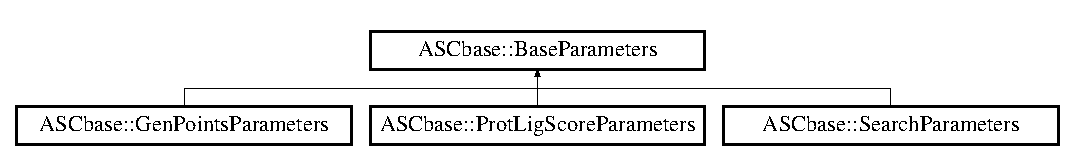
\includegraphics[height=1.72043cm]{classSimSite3D_1_1BaseParameters}
\end{center}
\end{figure}
\subsection*{Public Types}
\begin{CompactItemize}
\item 
\textbf{FATAL\_\-ERROR}\label{classSimSite3D_1_1BaseParameters_c80c7d6d1460ac21aee9af9e4adb27962ecf94b471dd1d92cfef939f1d8e5c5b}

\item 
\textbf{INVALID\_\-PARAMETER}\label{classSimSite3D_1_1BaseParameters_c80c7d6d1460ac21aee9af9e4adb27966a7dcbce394da1874589a864461ca96c}

\item 
\textbf{INITIALIZING}\label{classSimSite3D_1_1BaseParameters_c80c7d6d1460ac21aee9af9e4adb2796e0f14c6cff9f988fb50cd648984af4c8}

\item 
\textbf{DISPLAY\_\-HELP\_\-ONLY}\label{classSimSite3D_1_1BaseParameters_c80c7d6d1460ac21aee9af9e4adb2796009c052e63810d9249f5ba6d26733fcb}

\item 
\textbf{READY}\label{classSimSite3D_1_1BaseParameters_c80c7d6d1460ac21aee9af9e4adb27965688a5856aa9d26946abec13ed716dac}

\item 
enum \textbf{status\_\-t} \{ \par
\textbf{FATAL\_\-ERROR}, 
\textbf{INVALID\_\-PARAMETER}, 
\textbf{INITIALIZING}, 
\textbf{DISPLAY\_\-HELP\_\-ONLY}, 
\par
\textbf{READY}
 \}
\end{CompactItemize}
\subsection*{Public Member Functions}
\begin{CompactItemize}
\item 
status\_\-t \textbf{status} () const \label{classSimSite3D_1_1BaseParameters_39657de7d43af517724736e1c625546f}

\end{CompactItemize}
\subsection*{Static Public Member Functions}
\begin{CompactItemize}
\item 
static bool \textbf{get\_\-env\_\-var} (const std::string var, std::string $\ast$val)\label{classSimSite3D_1_1BaseParameters_f0c9884a0104f3b2e8595d401db60653}

\end{CompactItemize}
\subsection*{Public Attributes}
\begin{CompactItemize}
\item 
std::string \bf{dbase\_\-sites}\label{classSimSite3D_1_1BaseParameters_4812fa282e2ba266dbfa064182b594b9}

\begin{CompactList}\small\item\em Directory holding the database sitemaps. \item\end{CompactList}\item 
std::string \bf{dbase\_\-ligs}\label{classSimSite3D_1_1BaseParameters_d6b47ad4d8d7460817551da93171de4a}

\begin{CompactList}\small\item\em Directory holding the database ligands. \item\end{CompactList}\item 
std::string \bf{dbase\_\-prots}\label{classSimSite3D_1_1BaseParameters_fbb9b1185a994a991c0e68c30fa637b6}

\begin{CompactList}\small\item\em Directory holding the database proteins. \item\end{CompactList}\item 
std::string \bf{diverse\_\-sites}\label{classSimSite3D_1_1BaseParameters_89d38ef4448211e8ae3a63988e62f158}

\begin{CompactList}\small\item\em Directory holding the diverse sitemaps. \item\end{CompactList}\item 
std::string \bf{diverse\_\-ligs}\label{classSimSite3D_1_1BaseParameters_7431a50f3120b7f9f74026ad2c10b1a2}

\begin{CompactList}\small\item\em Directory holding ligands for diverse sitemaps. \item\end{CompactList}\item 
std::string \bf{proj\_\-output}\label{classSimSite3D_1_1BaseParameters_96522745ba23c6aac7d9258d65aac545}

\begin{CompactList}\small\item\em Directory to store results. \item\end{CompactList}\item 
std::string \bf{scratch\_\-dir}\label{classSimSite3D_1_1BaseParameters_96aa06a7fff08e400ec92d0ada56b786}

\begin{CompactList}\small\item\em Directory where SimSite3D can create temp files. \item\end{CompactList}\item 
std::string \textbf{install\_\-dir}\label{classSimSite3D_1_1BaseParameters_6fc273afb61ac03e5e733e704b9003d5}

\item 
bool \textbf{load\_\-surf\_\-files}\label{classSimSite3D_1_1BaseParameters_dd007d2ec07c2f19ed5eb847cede37e7}

\item 
bool \textbf{require\_\-min\_\-npts}\label{classSimSite3D_1_1BaseParameters_2cbb07424c917a0593f1d40ea08bec81}

\end{CompactItemize}
\subsection*{Protected Member Functions}
\begin{CompactItemize}
\item 
bool \textbf{load\_\-conf\_\-file} (std::string conf\_\-fname)\label{classSimSite3D_1_1BaseParameters_0bb99f45e58ded09c08f202dc662fb2c}

\item 
void \textbf{print\_\-version} (std::ostream \&out, std::string prog\_\-name)\label{classSimSite3D_1_1BaseParameters_dd81fff1ee86b790d0ee408cf3834116}

\end{CompactItemize}
\subsection*{Protected Attributes}
\begin{CompactItemize}
\item 
status\_\-t \bf{A\_\-status}\label{classSimSite3D_1_1BaseParameters_552075c2455c9ce279594f9d620de06a}

\begin{CompactList}\small\item\em Parameter status. \item\end{CompactList}\end{CompactItemize}
\subsection*{Private Member Functions}
\begin{CompactItemize}
\item 
void \textbf{load\_\-environment} ()\label{classSimSite3D_1_1BaseParameters_d14f824ff3778e6eeadc6f280e712fa8}

\item 
void \textbf{init\_\-str\_\-to\_\-var\_\-map} ()\label{classSimSite3D_1_1BaseParameters_2b6efe90e6fc04c12a708793b134c337}

\end{CompactItemize}
\subsection*{Private Attributes}
\begin{CompactItemize}
\item 
std::map$<$ std::string, std::string $\ast$ $>$ \textbf{A\_\-str\_\-to\_\-var}\label{classSimSite3D_1_1BaseParameters_d2d6dce8fdb7bc506d95de45aa545b07}

\end{CompactItemize}
\subsection*{Static Private Attributes}
\begin{CompactItemize}
\item 
static const std::string \bf{A\_\-fname} = \char`\"{}Base\-Parameters.C\char`\"{}\label{classSimSite3D_1_1BaseParameters_41d22522d6af1b42c1ae142bba6190ca}

\begin{CompactList}\small\item\em Name of source file. \item\end{CompactList}\end{CompactItemize}


\subsection{Detailed Description}
The order is to first read the \$ASCBASE\_\-INSTALL\_\-DIR environment variable. Second, parse \$ASCBASE\_\-INSTALL\_\-DIR/SimSite3D\-Soft\-Params/ascbase\_\-software.conf for system wide default values. Thirdly, check for any updated parameters in the environment. Finally, if load\_\-conf\_\-file is called by a derived class, the parsed values override all previously stored values. 



The documentation for this class was generated from the following files:\begin{CompactItemize}
\item 
Base\-Parameters.H\item 
Base\-Parameters.C\end{CompactItemize}
